\section{Introducción}

\indent \indent El objetivo de este trabajo práctico fue desarrollar un compositor de fórmulas matemáticas que tomara como entrada una versión simplicada del lenguaje utilzado por LATEX y produjera como salida un archivo SVG.\\
\indent \indent En las siguientes secciones se encontrarán detalles sobre el desarrollo de este trabajo práctico, instrucciones de uso y conclusiones.\\

\newpage

\section{Desarrollo}

\indent \indent La confección de este trabajo podría considerse dividida en dos etapas. \\
\indent La primer etapa corresponde a las modificaciones que se realizaron sobre la gramática del trabajo, con el fin de obtener una nueva gramática para la cual se pueda implementar un parser.
\indent La segunda etapa del trabajo significó la implementación del lexer, del parser y de la traducción propiamente dicha. Para ello, se utilizo la herramienta \textbf{ply}, que a partir de una ciertas reglas dadas por nosotros genera un parser LALR.\\

\subsection{Gramática}

\indent Se nos presentó una gramática ambigua a partir de la cual comenzar a trabajar con el fin implementar un traductor de cadenas de símbolos del lenguaje generado por dicha gramática a un fórmula matemática expresada en la sintaxis del formato SVG.
\indent La gramática original es la siguiente:

 \begin{equation}
    G = \langle \{ E\};\Sigma;P;E \rangle
 \end{equation}

\indent Donde $\Sigma = $ \{\_ , / , \{, \}, (, ) , \textit{l}, $\hat{}$ \} , \textit{l} es cualquier caracter a excepción de \_ , / , \{, \}, (, ) , , $\hat{}$  y \textbf{P} es el conjunto de producciones:

\begin{center}
 E $\rightarrow$ E E 
\\  $|$ E \textasciicircum E
\\  $|$ E \_ E
\\  $|$ E \textasciicircum E \_ E
\\  $|$ E \_ E \textasciicircum E
\\  $|$ E / E
\\  $|$ ( E )
\\  $|$ \{ E \} 
\\  $|$ $l$
\end{center}

\indent Al ser ambigua, debimos operar sobre la gramática para desambiguarla, teniendo en cuenta las siguientes restricciones:

\begin{itemize}
 \item La división es la de menor precedencia seguida de la concatencación.
  \item Tanto la división como la concatenación son asociativas a izquierda. Esto implica que la recursión las \textit{producciones} correspondientes será \textit{a izquierda}.
  \item El superíndice y supraíndice son no asociativos.
\end{itemize}

\indent Con estas cuestiones en mente, a partir de la gramática original se dio lugar a una nueva, no ambigua y que cumple las restricciones solicitadas:\\

\begin{equation}
    G = \langle \{ S, E, T, F, G\};\Sigma;P;S \rangle
 \end{equation}

\begin{center}
 S $\rightarrow$ E
\\ E $\rightarrow$ E / T
\\ E $\rightarrow$ T
\\ T $\rightarrow$ TF
\\ T $\rightarrow$ F
\\ F $\rightarrow$ G
\\ F $\rightarrow$ G\_G
\\ F $\rightarrow$ G\textasciicircum G
\\ F $\rightarrow$ G\textasciicircum G\_G
\\ F $\rightarrow$ G\_G\textasciicircum G
\\ G $\rightarrow$ \{ E\}
\\ G $\rightarrow$ (E)
\\ G $\rightarrow$ $l$
\end{center}

\indent Notar que la producción  S $\rightarrow$ E en realidad podría no estar. Se agregó a efectos de ser coherentes con la implementación que se hizo.\\ 

\subsection{Implementación}

\subsection{Lexer}

\indent \indent El lexer recibe una cadena y devuelve, en caso de poder traducir correctamente, la cadena tokenizada. Los tokens re reconocen haciendo uso de expresiones regulares. Se definieron los siguientes tokens:\\
\begin{itemize}
\item \textbf{SYMBOL}, que representa a cualquier caracter a excepción de \_ , / , \{, \}, (, ) y  $\hat{}$, es decir, representa el \textit{l} de la gramática. Se reconoce con la expresión regular \begin{verbatim}[^\_\^\{\}\(\)\/]\end{verbatim}
\item \textbf{LPARENT}, que representa el símbolo (. Se reconoce con la expresión regular \begin{verbatim} \(\end{verbatim}
\item \textbf{RPARENT}, que representa el símbolo ).  Se reconoce con la expresión regular \begin{verbatim} \) \end{verbatim}
\item \textbf{LBRACKET}, que representa el símbolo \{.  Se reconoce con la expresión regular \begin{verbatim} \{\end{verbatim}
\item \textbf{RBRACKET}, que representa el símbolo \}.  Se reconoce con la expresión regular \begin{verbatim} \}\end{verbatim}
\item \textbf{DIVIDE}, que representa el símbolo /.  Se reconoce con la expresión regular \begin{verbatim} \/\end{verbatim}
\item \textbf{CIRCUMFLEX}, que representa el símbolo $\hat{}$.  Se reconoce con la expresión regular \begin{verbatim} \^ \end{verbatim}
\item \textbf{UNDERSCORE}, que representa el símbolo \_.  Se reconoce con la expresión regular \begin{verbatim} \_ \end{verbatim}
\end{itemize}

\indent Aunque no sea necesario se decidió que el lexer ignore los espacios en blanco por cuestiones de comodidad.\\

\indent A continuación se provee el código del lexer. Se puede hallar en el archivo \textbf{lexer\_rules.py}:\\

\begin{verbatim}
tokens = [
    'SYMBOL',
    'LPARENT',
    'RPARENT',
    'LBRACKET',
    'RBRACKET',
    'DIVIDE',
    'CIRCUMFLEX',
    'UNDERSCORE'
]

t_LPARENT = r"\("
t_RPARENT = r"\)"
t_LBRACKET = r"\{"
t_RBRACKET = r"\}"
t_DIVIDE = r"\/"
t_CIRCUMFLEX = r"\^"
t_UNDERSCORE = r"\_"

def t_SYMBOL(token):
    r"[^\_\^\{\}\(\)\/]"
    return token

t_ignore = " \t\n"

def t_error(token):
    message = "Token desconocido:"
    message += "\ntype:" + token.type
    message += "\nvalue:" + str(token.value)
    message += "\nline:" + str(token.lineno)
    message += "\nposition:" + str(token.lexpos)
    raise Exception(message)

\end{verbatim}

\subsection{Parser}

\indent \indent El parser recibe una cadena tokenizada y devuelve un Abstract Syntax Tree de la cadena. Para cada producción de la gramática se define una función. Se crearon distintas clases que representan a los distintos posibles nodos del AST. Su implementación puede observarse en la sección correspondiente a la implementación de la traducción. El código del parser es el siguiente y se halla en el archivo \textbf{parser\_rules.py}:\\

\begin{verbatim}
from lexer_rules import tokens 
from expressions import Start, Divide, Concat, Underscore, Circumflex, 
                                CircumflexUnder, UnderCircumflex, Parenthesis, Symbol

def p_start_expression(subexpressions):
        'start : expression'
        subexpressions[0] = Start(subexpressions[1])
        
def p_expression_divide(subexpressions):
        'expression : expression DIVIDE term'
        subexpressions[0] = Divide(subexpressions[1], subexpressions[3])

def p_expression_term(subexpressions):
        'expression : term'
        subexpressions[0] = subexpressions[1]

def p_term_concat(subexpressions):
        'term : term factor'
        subexpressions[0] = Concat(subexpressions[1], subexpressions[2])

def p_term_factor(subexpressions):
        'term : factor'
        subexpressions[0] = subexpressions[1]

def p_factor_g(subexpressions):
        'factor : g'
        subexpressions[0] = subexpressions[1]

def p_factor_g_under_g(subexpressions):
        'factor : g UNDERSCORE g'
        subexpressions[0] = Underscore(subexpressions[1], subexpressions[3])

def p_factor_g_circum_g(subexpressions):
        'factor : g CIRCUMFLEX g'
        subexpressions[0] = Circumflex(subexpressions[1], subexpressions[3])

def p_factor_g_circum_g_under_g(subexpressions):
        'factor : g CIRCUMFLEX g UNDERSCORE g'
        subexpressions[0] = 
                     CircumflexUnder(subexpressions[1], subexpressions[3], subexpressions[5])

def p_factor_g_under_g_circum_g(subexpressions):
        'factor : g UNDERSCORE g CIRCUMFLEX g'
        subexpressions[0] = 
                     UnderCircumflex(subexpressions[1], subexpressions[3], subexpressions[5])

def p_g_bracket_expression(subexpressions):
        'g : LBRACKET expression RBRACKET'
        subexpressions[0] = subexpressions[2]

def p_g_parenthesis_expression(subexpressions):
        'g : LPARENT expression RPARENT'
        subexpressions[0] = Parenthesis(subexpressions[2])        

def p_g_symbol(subexpressions):
        'g : SYMBOL'
        subexpressions[0] = Symbol(subexpressions[1])

def p_error(subexpressions):
    raise Exception("Syntax error.")
\end{verbatim}

\subsection{Traductor}
\indent \indent  La operatoria para traducir se compone de dos partes.\\
\indent La primera, \textbf{operate} se encarga de calcular a partir del AST los valores de los atributos para cada nodo. Para hacerlo, se recorre el árbol a partir del nodo de inicio.\\
\indent La idea es que en la llamada a \textit{operate} para un nodo dado, se computen en primer lugar los valores que necesitan los nodos hijos para poder calcular sus atributos llamando dentro de este contexto a sus \textit{operate}.\\
\indent Notemos que en algunos casos como la división, los subíndices y los superíndices no alcanza con llamar al \textit{operate} de cada hijo para terminar de computar sus atributos sino que además es necesario hacer más cálculos que permiten moverlos de posición de manera que se pueda visualizar correctamente la fórmula.\\
\indent Como se puede ver, para cada nodo del AST se llama una única vez a \textbf{operate}. Luego, ejecutando \textit{operate} al nodo de inicio, que es de la clase \textit{Start}, se calculan los valores de los atributos de cada nodo necesarios para la traducción a SVG de toda la cadena.\\
\indent \indent La segunda parte, \textbf{translate}, se corresponde a la traducción propiamente dicha. Esta parte también opera con el AST, al que asume que ya se le aplicó \textbf{operate}, y en base a los valores de los atributos calculados en dicha operación genera la traducción en el formato SVG, sintetizando la traducción en el atributo \textbf{translation}.\\
\indent Se crearon distintas clases que representan a los posibles nodos del AST:
\begin{itemize}
\item \textbf{Start}, representa al nodo que se obtiene de aplicar la producción inicial  S $\rightarrow$ E . Posee un atributo \textit{child} que representa al nodo hijo.
\item \textbf{Divide}, representa al nodo que se obtiene de aplicar la producción E $\rightarrow$ $E_2$ / T . Posee un atributo \textit{left} que señala al nodo hijo que corresponde al $E_2$ y un atributo \textit{right} que indica el nodo hijo que corresponde a T.
\item \textbf{Concat}, representa al nodo que se obtiene de aplicar la producción T $\rightarrow$ $T_2$F . Posee un atributo \textit{left} que señala al nodo hijo que corresponde al $T_2$ y un atributo \textit{right} que indica el nodo hijo que corresponde a F.
\item \textbf{Underscore}, representa al nodo que se obtiene de aplicar la producción F$\rightarrow$ G\_$G_2$. Posee un atributo \textit{left} que señala al nodo hijo que corresponde al G (la raíz) y un atributo \textit{right} que indica el nodo hijo que corresponde a $G_2$ (el subíndice).
\item \textbf{Circumflex}, representa al nodo que se obtiene de aplicar la producción F$\rightarrow$ G\textasciicircum$G_2$. Posee un atributo \textit{left} que señala al nodo hijo que corresponde al G (la raíz) y un atributo \textit{right} que indica el nodo hijo que corresponde a $G_2$ (el superíndice).
\item \textbf{UnderCircumflex}, representa al nodo que se obtiene de aplicar la producción F $\rightarrow$ G\_$G_2$\textasciicircum $G_3$. Posee un atributo \textit{first} que señala al nodo hijo que corresponde al G (la raíz), un atributo \textit{second} que indica el nodo hijo que corresponde a $G_2$ (el subíndice) y un atributo \textit{third} que indica el nodo hijo que corresponde a $G_3$(el superíndice).
\item \textbf{CircumflexUnder}, representa al nodo que se obtiene de aplicar la producción F $\rightarrow$ G\textasciicircum $G_2$\_$G_3$. Posee un atributo \textit{first} que señala al nodo hijo que corresponde al G (la raíz), un atributo \textit{second} que indica el nodo hijo que corresponde a $G_2$ (el superíndice) y un atributo \textit{third} que indica el nodo hijo que corresponde a $G_3$(el subíndice).
\item \textbf{Parenthesis}, representa al nodo que se obtiene de aplicar la producción G $\rightarrow$ (E). Posee un atributo \textit{child} que representa al nodo hijo que corresponde a E.
\item \textbf{Symbol}, representa al nodo que se obtiene de aplicar la producción G $\rightarrow$ $l$. Posee un atributo \textit{value} que señala el valor del terminal $l$ y siempre es una hoja, es decir que no tiene nodos hijo.
\end{itemize}

\indent \indent Notemos que las demás producciones, E $\rightarrow$ T, T $\rightarrow$ F, F $\rightarrow$ G, G $\rightarrow$ \{ E\}, no proveen ninguna clase de nodo nueva.\\


\indent Además, cada una de las clases mencionadas posee los siguiente atributos:

\begin{itemize}
\item  \textbf{x} e \textbf{y} que describen las coordenadas de los nodos y son atributos heredados.
\item \textbf{width} y \textbf{height} que representan el ancho y el alto de la subfórmula de cada nodo y son atributos sintetizados.
\item \textbf{scale} que es un atributo heredado que señala la escala de la subfórmula del nodo.
\item \textbf{ht} y \textbf{dp} son atributos que representan, respectivamente y pensando en cada símbolo como dentro de una caja, la distancia entre la línea de base y el tope de la caja y la distancia entre la línea de base y el fondo de la caja. De esta manera, se deduce que la altura del nodo (el atributo \textit{height}) se corresponde con la suma de estos dos atributos. La idea se obtuvo del capítulo 5 de la segunda edición del \textit{Compilers, Principles, Techniques, \& Tools} de Aho, Lam, Sethi y Ullman.
\item \textbf{maxY} y \textbf{minHScale} son atributos que se utilizan para los casos donde hay muchos subíndices seguidos y que nos permiten en efecto reflejar la no asociatividad del subíndice. \textit{maxY} refleja la posición que más debajo se encuentra en el nodo raíz y \textit{minHScale}, el tamaño del subíndice que más debajo se ha hallado en la raíz. De esta manera, sabemos dónde y con qué escala ubicar un nuevo subíndice.
\item \textbf{minY} y \textbf{minLScale} son atributos análogos a \textit{maxY} y \textit{minHScale} pero para el caso donde hay mucho superíndices seguidos. \textit{minY} refleja, entonces, la posición que más arriba se encuentra en el nodo raíz y \textit{minLScale}, el tamaño del superíndice que más arriba se ha hallado en la raíz.
\item \textbf{translation} es un atributo sintetizado donde se va calculando la traducción a SVG de la fórmula. \textbf{translate} se encarga de computarlo.
\end{itemize}

\indent A continuación se provee el código correspondiente a esta sección. Corresponde al archivo \textbf{expressions.py}. Recomendamos leer los comentarios en el código para comprender con más facilidad el programa.
\begin{verbatim}
#constantes que se utilizan para inicializar atributos
DEFAULT_SCALE = 1
DEFAULT_HT = 0.8
DEFAULT_DP = 0.2
DEFAULT_X = 0
DEFAULT_Y = 0
DEFAULT_HEIGHT = 1
DEFAULT_WIDTH = 0.6

#funcion que escala el nodo pasa por parametro por el scale indicado
def scale(node, scale):
  node.scale = scale
  node.height = node.height * scale
  node.dp = node.dp * scale
  node.ht = node.ht * scale
  node.width = node.width * scale
  node.minHScale = node.minHScale * scale
  node.minLScale = node.minLScale * scale

#funcion que mueve verticalmente un nodo y todos sus nodos hijos
def moveY(node, y):
  node.y += y
  node.minY += y
  node.maxY += y
  for c in node.children:
    moveY(c, y)

#funcion que mueve horizontalmente un nodo y todos sus nodos hijos
def moveX(node, x):
  node.x += x
  for c in node.children:
    moveX(c, x)

class Start(object):
  def __init__(self, child):
    self.child = child
    self.x = DEFAULT_X
    self.y = 1
    self.scale = DEFAULT_SCALE
    self.dp = DEFAULT_DP
    self.ht = DEFAULT_HT
    self.height = DEFAULT_HEIGHT
    self.minY = 1
    self.maxY = 1
    self.minHScale = DEFAULT_SCALE
    self.minLScale = DEFAULT_SCALE
    self.children = [child]

  #para debugging
  def name(self):
    return self.child.name()

  def operate(self):
    #escalamos el nodo hijo
    scale(self.child, self.scale)

    #seteamos las posiciones del nodo hijo 
    #en este caso se corresponden con la del nodo padre

    self.child.x = self.x
    self.child.y = self.y

    #computamos los atributos del nodo hijo

    self.child.operate()

    #el ht y el dp se corresponden con el del nodo hijo

    self.dp = self.child.dp
    self.ht = self.child.ht

    #ht + dp dan la altura del nodo

    self.height = self.dp + self.ht

  def translate(self):

    #escribimos el header del svg

    self.translation =  '<?xml version="1.0" standalone="no"?>\n'
    self.translation += '<!DOCTYPE svg PUBLIC "-//W3C//DTD SVG 1.1//EN"\n'
    self.translation += '"http://www.w3.org/Graphics/SVG/1.1/DTD/svg11.dtd">\n'
    self.translation += '<svg xmlns="http://www.w3.org/2000/svg" version="1.1">\n'

    #bajamos tanto como necesitemos la formula para que se vea por completo en pantalla
    #el scale es arbitrario, suficiente para 
    #visualizar correctamente la formula sin agrandarla demasiado

    self.translation +=
      '<g transform="translate(20,' + 
            str((self.ht-self.y + 3) * 15) + ') scale(15)" font-family="Courier">\n'
    
    #traducimos el nodo hijo

    self.translation += self.child.translate()

    #cerramos el grupo

    self.translation +='</g>\n'
    self.translation += '</svg>'
    return self.translation

class Divide(object):
  def __init__(self, left, right):
    self.left = left
    self.right = right
    self.width  = DEFAULT_WIDTH
    self.height = DEFAULT_HEIGHT
    self.x = DEFAULT_X
    self.y = DEFAULT_Y
    self.scale = DEFAULT_SCALE
    self.dp = DEFAULT_DP
    self.ht = DEFAULT_HT
    self.minY = 1
    self.maxY = 1
    self.minHScale = DEFAULT_SCALE
    self.minLScale = DEFAULT_SCALE
    self.children = [left, right]

  #para debugging
  def name(self):

    return self.left.name() + "/" + self.right.name()

  def operate(self):

    #primero escalamos los nodos hijos
    #en este caso las escalas se mantienen en los nodos hijos

    scale(self.left, self.scale)
    scale(self.right, self.scale)
    
    #seteamos las primeras posiciones para los nodos hijos
    #inicialmente son las del nodo padre,
    #luego se moveran los nodos donde corresponda

    self.left.x = self.x
    self.left.y = self.y 
    self.right.x = self.x
    self.right.y = self.y

    #computamos los atributos de los nodos hijos

    self.left.operate()
    self.right.operate()
    
    #actualizamos el ht y el dp del nodo
    #el ht del nodo es la altura del numerador mas 
    #aproximadamente un 40% mas de la escala 
    #pues debe estar arriba de la linea de division

    self.ht = self.left.height + 0.40 * self.scale

    #el dp del nodo depende de la altura del denominador mas
    #aproximamente un 28% de la escala puesto que 
    #debe estar debajo de la linea de division

    self.dp = self.right.height + 0.28 * self.scale
    
    #la anchura es la maxima anchura de los hijos

    self.width = max(self.left.width, self.right.width)

    #reubicamos el numerador por arriba de la linea de division,
    #tanto como se haya pasado y un poco mas

    moveY(self.left, -self.left.dp - 0.50 * self.scale)
    
    #reubicamos el denominador por debajo de la linea de division

    moveY(self.right, self.right.ht + 0.28*self.scale)

    #calculamos al altura del nodo
    self.height = self.dp + self.ht

    #calculamos el centro de la division y centramos los nodos hijos
    #calculo el centro del nodo

    center = (self.x + (self.x + self.width))/2

    #calculo el centro del denominador

    rightCenter = (self.right.x + (self.right.x + self.right.width))/2

    #calculo el centro del numerador

    leftCenter = (self.left.x + (self.left.x + self.left.width))/2

    #movemos horizontalmente al numerador y al denominador
    #por la distancia que separa a sus centros del centro del nodo padre

    moveX(self.left, abs(leftCenter - center))
    moveX(self.right, abs(rightCenter - center))


      
    
  def translate(self):

    #traducimos el numerador

    self.translation = self.left.translate()

    #pintamos la linea de division

    self.translation += 
      '\t<line x1="' + str(self.x) + '" y1="' + 
          str(self.y - 0.28 * self.scale) + '" '
    self.translation += 
      'x2="' + str(self.x + self.width) +
        '" y2="' + str(self.y -  0.28 * self.scale) + '" '
    self.translation +='stroke-width="0.03" stroke="black"/>\n'
    
    #finalmente traducimos el denominador

    self.translation += self.right.translate()
    return self.translation



class Concat(object):
  def __init__(self, left, right):
    self.scale = DEFAULT_SCALE
    self.height = DEFAULT_HEIGHT
    self.left = left
    self.right = right
    self.x = DEFAULT_X
    self.y = DEFAULT_Y
    self.width = DEFAULT_WIDTH
    self.dp = DEFAULT_DP
    self.ht = DEFAULT_HT
    self.minY = 1
    self.maxY = 1
    self.minHScale = DEFAULT_SCALE
    self.minLScale = DEFAULT_SCALE
    self.children = [left, right]
    
  #para debugging
  def name(self):
    return self.left.name() + " " + self.right.name()

  def operate(self):

    #escalamos los nodos hijos
    #las escalas son las del nodo padre

    scale(self.left, self.scale)
    scale(self.right, self.scale)

    #seteamos la posicion de los nodos hijo 
    #mas a la izquierda y computamos sus atributos.

    self.left.x = self.x
    self.left.y = self.y
    self.left.operate()

    #seteamos la posicion del nodo derecho, 
    #teniendo en cuenta que debe ubicarse luego del izquierdo,
    #y computamos sus atributos

    self.right.x = self.left.x + self.left.width
    self.right.y = self.y
    self.right.operate()

    #la anchura del nodo es la suma de las anchuras de los nodos hijos

    self.width = self.left.width + self.right.width

    #actualizamos ht y dp y con ellos calculamos la altura del nodo
    #el dp y el ht corresponde a los mayores dp y ht hallados en los hijos

    self.dp = max(self.left.dp, self.right.dp)
    self.ht = max(self.left.ht, self.right.ht)
    self.height = self.dp + self.ht
    

  def translate(self):

    #traducimos el hijo izquierdo y a continuacion el hijo derecho

    self.translation = self.left.translate() + self.right.translate()
    return self.translation

class Underscore(object):
  def __init__(self, left, right):
    self.x = DEFAULT_X
    self.y = DEFAULT_Y
    self.left = left
    self.right = right
    self.height = DEFAULT_HEIGHT
    self.scale = DEFAULT_SCALE
    self.width = DEFAULT_WIDTH
    self.dp = DEFAULT_DP
    self.ht = DEFAULT_HT
    self.minY = 1
    self.maxY = 1
    self.minHScale = DEFAULT_SCALE
    self.minLScale = DEFAULT_SCALE
    self.children = [left, right]
    
  #para debugging
  def name(self):
    return self.left.name() + "_" + self.right.name()

  def operate(self):

    #escalamos el nodo raiz

    scale(self.left, self.scale)

    #seteamos la posicion del nodo hijo raiz
    #corresponde con la posicion calculada para el nodo padre
    #y calculamos sus atributos

    self.left.x = self.x
    self.left.y = self.y
    self.left.operate()

    #escalo el subindice a partir del menor 
    #tamanio encontrado en el nodo raiz

    scale(self.right,self.left.minHScale * 0.7)

    #computo sus atributos del nodo indice
    #para la posicion vertical hago uso del mayor 'y' 
    #que puede encontrar en el nodo raiz
    #y lo bajo un poco mas de acuerdo al menor 
    #tamanio hallado en el nodo raiz y al ht del indice

    self.right.x = self.x + self.left.width
    self.right.operate()
    moveY(self.right, self.left.maxY + self.right.ht)

    #actualizamos dp, height, width, maxY, minHScale con lo que calculamos del nodo hijo
    #el ht no cambia, porque la formula crece para "abajo"
    #el dp corresponde al de la raiz mas la altura del indice 
    #menos aproximadamente un 25% de la minima escala encontrada en la raiz
    #para no bajar demasiado el indice

    self.dp = self.left.dp + self.right.height - 0.25 * self.left.minHScale

    #el maximo 'y' ahora corresponde al maximo 'y' del indice
    #la minima escala tambien corresponde con la minima escala del indice

    self.maxY = self.right.maxY
    self.minHScale = self.right.minHScale

    #el ancho es la suma de los anchos de la raiz y del indice

    self.width = self.left.width + self.right.width
    self.height = self.dp + self.ht
    
  def translate(self):

    #primero traducimos el nodo raiz y a continuacion el subindice

    self.translation = self.left.translate()
    self.translation += self.right.translate()
    return self.translation

class Circumflex(object):
  def __init__(self, left, right):
    self.left = left
    self.right = right
    self.scale = DEFAULT_SCALE
    self.height = DEFAULT_HEIGHT
    self.x = DEFAULT_X
    self.y = DEFAULT_Y
    self.width = DEFAULT_WIDTH
    self.dp = DEFAULT_DP
    self.ht = DEFAULT_HT
    self.minY = 1
    self.maxY = 1
    self.minHScale = DEFAULT_SCALE
    self.minLScale = DEFAULT_SCALE
    self.children = [left, right]

  #para debugging
  def name(self):
    return self.left.name() + "^" + self.right.name()

  def operate(self):

    #escalamos el nodo raiz
    scale(self.left, self.scale)

    #seteamos la posicion del nodo hijo raiz
    #la posicion es la del nodo padre
    #y calculamos sus atributos

    self.left.x = self.x
    self.left.y = self.y
    self.left.operate()

    #escalo el superindice a partir del menor tamanio encontrado en el nodo raiz

    scale(self.right,self.left.minLScale * 0.7)
    
    #seteo las posiciones del superindice y computo sus atributos

    self.right.x = self.x + self.left.width
    self.right.operate()

    #para la posicion vertical hago uso del menor 'y' 
    #que pude encontrar en el nodo raiz
    #y lo subo un poco mas de acuerdo 
    #al menor tamanio hallado en el nodo raiz y
    #y de acuerdo a cuanto se pasa por debajo 
    #de linea de base del superindice que aparece mas arriba

    moveY(self.right, self.left.minY  - self.right.dp - (0.45 * self.left.minLScale))


    #actualizamos ht, height, width, maxY, minHScale 
    #con lo que calculamos del nodo hijo
    #el dp no hace falta modificarlo puesto que la formula crece para "arriba"
    #el ht es el de la raiz mas altura del superindice menos
    #aproximadamente un 30% del la minima escala para superindices hallada

    self.ht = self.left.ht + self.right.height - 0.30 * self.left.minLScale
    
    #el minimo 'y' es el del superindice
    
    self.minY = self.right.minY
    
    #la minima escala es la del superindice
    
    self.minLScale = self.right.minLScale
    
    #el ancho es la suma de los anchos de la raiz y del superindice
    
    self.width = self.left.width + self.right.width
    self.height = self.dp + self.ht
  
  def translate(self):
    
    #primero traducimos el nodo raiz y a continuacion el superindice
    
    self.translation = self.left.translate()
    self.translation += self.right.translate()
    return self.translation

class CircumflexUnder(object):
  def __init__(self, first, second, third):
    self.scale = DEFAULT_SCALE
    self.x = DEFAULT_X
    self.y = DEFAULT_Y
    self.width = DEFAULT_WIDTH
    self.height = DEFAULT_HEIGHT
    self.dp = DEFAULT_DP
    self.ht = DEFAULT_HT
    self.minY = 1
    self.maxY = 1
    self.minHScale = DEFAULT_SCALE
    self.minLScale = DEFAULT_SCALE
    self.first = first
    self.second = second
    self.third = third
    self.children = [first, second, third]

  #para debugging
  def name(self):
    return self.first.name() + "^" + self.second.name() + "_" + self.third.name()

  def operate(self):
    
    #escalamos el nodo raiz
    
    scale(self.first, self.scale)

    #seteamos la posicion del nodo hijo raiz
    #la posicion se corresponde con la del nodo padre
    #y calculamos sus atributos
    
    self.first.x = self.x
    self.first.y = self.y
    self.first.operate()

    #escalo el superindice a partir del menor 
    #tamanio encontrado de superindices en el nodo raiz
    #escalo el subindice a partir del menor 
    #tamanio encontrado de subindices en el nodo raiz

    scale(self.second, self.first.minLScale * 0.7)
    scale(self.third, self.first.minHScale * 0.7)

    #seteo las posiciones del superindice y del subindice y computo sus atributos
    #luego del computo se moveran verticalmente como corresponda

    self.second.x = self.x + self.first.width
    self.third.x = self.x + self.first.width
    self.second.operate()
    self.third.operate()
    
    #para la posicion vertical del superindice hago uso del menor 'y' 
    #que pude encontrar en el nodo raiz
    #y lo subo un poco mas de acuerdo al menor tamanio 
    #hallado para superindices en el nodo raiz y
    #y de acuerdo a cuanto se pasa por debajo de la 
    #linea de base del superindice que aparece mas arriba
    #para la posicion vertical del subindice hago uso del mayor 'y' 
    #que puede encontrar en el nodo raiz
    #y lo bajo un poco mas de acuerdo al menor tamanio 
    #hallado para subindices en el nodo raiz y al ht del indice

    moveY(self.second, self.first.minY  - self.second.dp - (0.45 * self.first.minLScale))
    moveY(self.third, self.first.maxY + self.third.ht)

    #actualizamos ht, dp, height, width, maxY, minHScale, minY, minLScale 
    #con lo que calculamos de los nodos hijos
    #el ht es el de la raiz mas la altura del superindice menos
    #aproximadamente un 30% del la minima escala para superindices hallada

    self.ht = self.first.ht + self.second.height - 0.30 * self.first.minLScale

    #el dp corresponde al de la raiz mas la altura del subindice 
    #menos aproximadamente un 25% de la minima 
    #escala para subindices encontrada en la raiz
    
    self.dp = self.first.dp + self.third.height - 0.25 * self.first.minHScale
    
    #el minimo 'y' es el del superindice
    
    self.minY = self.second.minY
    
    #la minima escala para superindices es la minima 
    #escala hallada en el superindice
    
    self.minLScale = self.second.minLScale
    
    #el maximo 'y' ahora corresponde al maximo 'y' del subindice
    
    self.maxY = self.third.maxY
    
    #la minima escala para subindices tambien corresponde 
    #con la minima escala hallada en el subindice
    
    self.minHScale = self.third.minHScale
    
    #el ancho es la suma del ancho de la raiz mas 
    #la maxima anchura entre el superindice y el subindice
    
    self.width = self.first.width + max(self.second.width, self.third.width)
    self.height = self.ht + self.dp

  def translate(self):

    #traducimos en primer lugar la raiz
    #luego traducimos el superindice
    #finalmente traducimos el subindice
    
    self.translation = self.first.translate()
    self.translation += self.second.translate()
    self.translation += self.third.translate()
    return self.translation


class UnderCircumflex(object):
  def __init__(self, first, second, third):
    self.scale = DEFAULT_SCALE
    self.x = DEFAULT_X
    self.y = DEFAULT_Y
    self.width = DEFAULT_WIDTH
    self.height = DEFAULT_HEIGHT
    self.dp = DEFAULT_DP
    self.ht = DEFAULT_HT
    self.minY = 1
    self.maxY = 1
    self.minHScale = DEFAULT_SCALE
    self.minLScale = DEFAULT_SCALE
    self.first = first
    self.second = second
    self.third = third
    self.children = [first, second, third]

  #para debugging
  def name(self):
    return self.first.name() + "_" + self.second.name() + "^" + self.third.name()

  def operate(self):

    #escalamos el nodo raiz
    
    scale(self.first, self.scale)

    #seteamos la posicion del nodo hijo raiz
    #la posicion se corresponde con la del nodo padre
    #y calculamos sus atributos
    
    self.first.x = self.x
    self.first.y = self.y
    self.first.operate()

    #escalo el superindice a partir del menor 
    #tamanio encontrado de superindices en el nodo raiz
    #escalo el subindice a partir del menor 
    #tamanio encontrado de subindices en el nodo raiz

    scale(self.third, self.first.minLScale * 0.7)
    scale(self.second, self.first.minHScale * 0.7)

    #seteo las posiciones del superindice y del subindice y computo sus atributos
    #luego del computo se moveran verticalmente como corresponda

    self.third.x = self.x + self.first.width
    self.second.x = self.x + self.first.width
    self.third.operate()
    self.second.operate()

    #para la posicion vertical del superindice hago uso del menor 'y' 
    #que pude encontrar en el nodo raiz
    #y lo subo un poco mas de acuerdo al menor tamanio 
    #hallado para superindices en el nodo raiz y
    #y de acuerdo a cuanto se pasa por debajo de la 
    #linea de base del superindice que aparece mas arriba
    #para la posicion vertical del subindice hago uso del mayor 'y' 
    #que puede encontrar en el nodo raiz
    #y lo bajo un poco mas de acuerdo al menor tamanio hallado 
    #para subindices en el nodo raiz y al ht del indice
    
    moveY(self.third, self.first.minY  - self.third.dp - (0.45 * self.first.minLScale))
    moveY(self.second, self.first.maxY + self.second.ht)

    #actualizamos ht, dp, height, width, maxY, minHScale, minY, minLScale 
    #con lo que calculamos de los nodos hijos
    #el ht es el de la raiz mas la altura del superindice menos
    #aproximadamente un 30% del la minima escala para superindices hallada
    
    self.ht = self.first.ht + self.third.height - 0.30 * self.first.minLScale
    
    #el dp corresponde al de la raiz mas la altura del subindice 
    #menos aproximadamente un 25% de 
    #la minima escala para subindices encontrada en la raiz
    
    self.dp = self.first.dp + self.second.height - 0.25 * self.first.minHScale
    
    #el minimo 'y' es el del superindice
    
    self.minY = self.third.minY
    
    #la minima escala para superindices es 
    #la minima escala hallada en el superindice
    
    self.minLScale = self.third.minLScale
    
    #el maximo 'y' ahora corresponde al maximo 'y' del subindice
    
    self.maxY = self.second.maxY
    
    #la minima escala para subindices tambien 
    #corresponde con la minima escala hallada en el subindice
    
    self.minHScale = self.second.minHScale
    
    #el ancho es la suma del ancho de la raiz 
    #mas la maxima anchura entre el superindice y el subindice

    self.width = self.first.width + max(self.second.width, self.third.width)
    self.height = self.ht + self.dp

  def translate(self):

    #traducimos en primer lugar la raiz
    #luego traducimos el subindice
    #finalmente traducimos el superindice
    
    self.translation = self.first.translate()
    self.translation += self.second.translate()
    self.translation += self.third.translate()
    return self.translation    

class Parenthesis(object):
  def __init__(self, child):
    self.scale = DEFAULT_SCALE
    self.x = DEFAULT_X
    self.y = DEFAULT_Y
    self.width = DEFAULT_WIDTH
    self.height = DEFAULT_HEIGHT
    self.dp = DEFAULT_DP
    self.ht = DEFAULT_HT
    self.minY = 1
    self.maxY = 1
    self.minHScale = DEFAULT_SCALE
    self.minLScale = DEFAULT_SCALE
    self.child = child
    self.children = [child]
  
  #para debugging  
  def name(self):
    return "(" + self.child.name() + ")"

  def operate(self):

    #escalamos el nodo hijo
    
    scale(self.child, self.scale)

    #horizontalmente movemos el nodo hijo 
    #para dejar lugar al parentesis que abre
    #la posicion vertical del hijo es la del nodo
    
    self.child.x = self.x + self.scale * 0.6
    self.child.y = self.y

    #computamos los atributos del nodo hijo
    self.child.operate()

    #la anchura del nodo es la del hijo 
    #mas el ancho del parentesis que abre 
    #mas el ancho del parentesis que cierra
    
    self.width = self.child.width + (2 * self.scale * 0.6)

    #actualizamos los ht y dp y la altura del nodo
    #corresponden a los hy y dp del hijo
    
    self.dp = self.child.dp 
    self.ht = self.child.ht  
    self.height = self.dp + self.ht

  def translate(self):
    #escala es un valor que se utiliza para escalar los 
    #parentesis de manera tal que cubran toda la formula 
    #y para reubicarlos. se lo divide por self.scale 
    #para contrarrestar el efecto del font-size al transformar
    # el 1.33 es un valor que 
    #probando descubrimos que parece funcionar correctamente 

    escala = self.height * 1.33 / self.scale
    
    #se escribe el parentesis que abre.
    
    self.translation = '\t<text x="0" y="0" font-size="' + str(self.scale) + '" transform="'
    
    #verticalmente se ubica un poco por encima 
    #de donde empieza el nodo hijo,
    #dado que el simbolo de parentesis 
    #se escribe un poco por debajo en la fuente elegida
    #se lo escala por el valor escala calculado

    self.translation += 
      'translate(' + str(self.x) + ',' + 
          str(self.y + self.dp - 0.18 * escala) + ') scale(1,' + str(escala) + ')">(</text>\n'
    
    #traducimos el nodo hijo

    self.translation += self.child.translate()

    #escribimos el parentesis que cierra.
    #idem al partentesis  que abre,
    # con la excepcion de que verticalmente 
    #aparece mas a la derecha tanto como anchura tenga el nodo hijo

    self.translation += '\t<text x="0" y="0" font-size="' + str(self.scale) + '" transform="'
    self.translation += 
      'translate(' + str(self.x + self.child.width + self.scale * 0.6) + 
        ',' + str(self.y + self.dp - 0.18 * escala) + ') scale(1,'+ str(escala) +')">)</text>\n'
    return self.translation

class Symbol(object):
  def __init__(self, value):
    self.value = value
    self.scale = DEFAULT_SCALE
    self.width = DEFAULT_WIDTH
    self.height = DEFAULT_HEIGHT
    self.dp = DEFAULT_DP
    self.ht = DEFAULT_HT
    self.x = DEFAULT_X
    self.y = DEFAULT_Y
    self.minY = 1
    self.maxY = 1
    self.minHScale = DEFAULT_SCALE
    self.minLScale = DEFAULT_SCALE
    self.children = []

  #para debugging
  def name(self):
    return str(self.value)

  def operate(self):
    #calculo los maxY y minY para el caso en el 
    #que el nodo padre es un subindice o superindice
    #o alguna combinacion de subindice y superindices 
    #como undercircumflex o circumflexunder
    
    self.maxY = self.y
    self.minY = self.y
    pass

  def translate(self):
    #traduzco el nodo de acuerdo a los 
    #atributos que se computaron en operate
    
    return '\t<text x="' + str(self.x) + '" y="' + 
      str(self.y) +'" font-size="' + str(self.scale) + '">' + str(self.value) + '</text>\n'

\end{verbatim}


\newpage

\section{Algunas Traducciones de Ejemplo}

\begin{figure}[H]
      \begin{centering}
        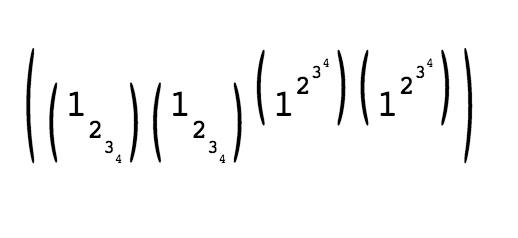
\includegraphics{imgs/a}
        \caption{$((\{\{1\_2\}\_3\}\_4)(1\_\{2\_\{3\_4\}\})(\{\{1\wedge2\}\wedge3\}\wedge4)(1\wedge\{2\wedge\{3\wedge4\}\}))$}
       \end{centering}
\end{figure}

\indent Este ejemplo lo queremos utilizar para hacer notar un par de cuestiones. La primera de ellas es demostrar la no asocitividad del subíndice y del superíndice. La segunda tiene que ver con los paréntesis. Como se puede notar, los parentésis de las fórmulas que son una concatenación de subíndices y las de aquellas que son una concatenación de superíndices no están alineados, y puede parecer raro a la vista. Nosotros creemos, sin embargo, que así como se muestra es cómo se debería ver. Tal visualización tiene sentido, dado que los subíndices hacen crecer la fórmula hacia abajo, mientras que los superíndices la hacen crecer para arriba. Luego, para cubrir correctamente la fórmula, el paréntesis debe ubicarse por debajo en el caso de los subíndices en comparación del caso de los superíndices. Otro detalle que parece confirmar nuestro pensamiento es que las raíces principales de la fórmulas (los 1's), están alineados sobre la misma línea de base.\\

\begin{figure}[H]
      \begin{centering}
        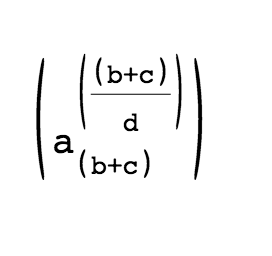
\includegraphics{imgs/b}
        \caption{$(a\wedge(\{(b+c)\}/d)\_(b+c))$}
       \end{centering}
\end{figure}
\begin{figure}[H]
      \begin{centering}
        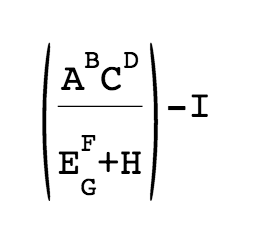
\includegraphics{imgs/c}
        \caption{$(A\wedge BC\wedge D/E\wedge F\_G+H)-I$}
       \end{centering}
\end{figure}
\begin{figure}[H]
      \begin{centering}
        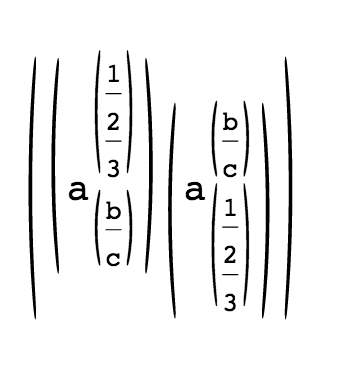
\includegraphics{imgs/d}
        \caption{$((a\wedge(1/2/3)\_(b/c))(a\wedge(b/c)\_(1/2/3)))$}
       \end{centering}
\end{figure}

\indent En la figura anterior se puede observar nuevamente esta disparidad entre los paréntesis. De vuelta, consideramos que esto tiene sentido puesto que la subfórmula de la izquierda termina más arriba que la de la derecha, que, a su vez, termina más por debajo que la de la izquierda.\\

\begin{figure}[H]
      \begin{centering}
        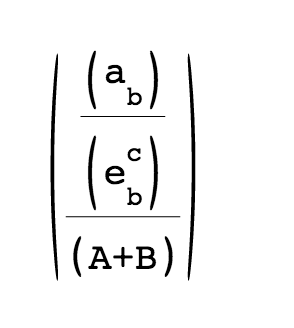
\includegraphics{imgs/e}
        \caption{$((a\_b)/(e\_b\wedge c)/(A + B))$}
       \end{centering}
\end{figure}
\begin{figure}[H]
      \begin{centering}
        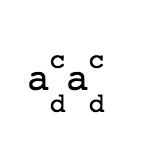
\includegraphics{imgs/f}
        \caption{${a\wedge c\_d}{a\_d\wedge c}$}
       \end{centering}   
\end{figure}

\indent La figura 6 tiene como objetivo mostrar que es equivalente en la traducción aplicar primero el subíndice y luego el superíndice o viceversa.\\

\begin{figure}[H]
      \begin{centering}
        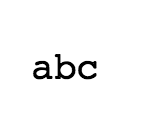
\includegraphics{imgs/g}
        \caption{$abc$}
       \end{centering}
\end{figure}
\begin{figure}[H]
      \begin{centering}
        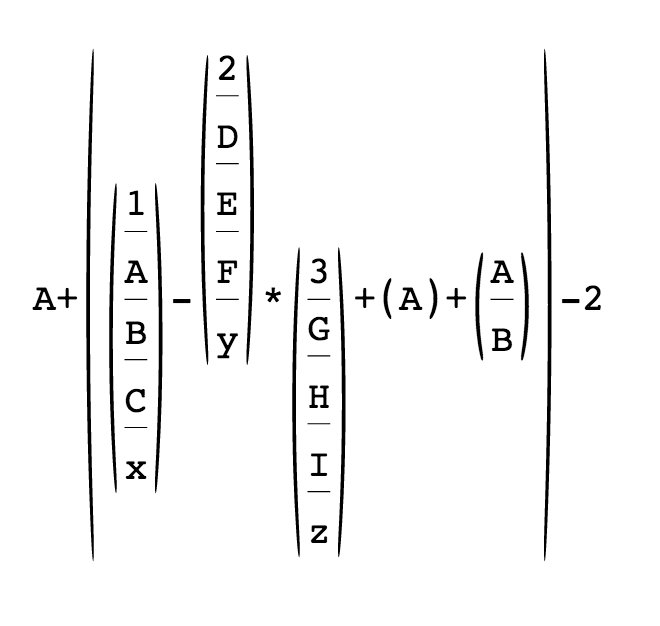
\includegraphics{imgs/h}
        \caption{$A+((\{1/A\}/\{B/C/x\})-(2/D/E/F/y)*(3/\{G/H/I/z\})+(A)+(A/B))-2$}
       \end{centering}
\end{figure}

\indent La figura anterior nos parece importante puesto que demuestra cómo afecta a la traducción la asociatividad de la división, algo que queda en evidencia con la disparidad en la lineación de la división.\\
\indent Como se puede observar, para la primer división parece que la operación dominante y que determina dónde se ubica la subfórmula es la que se produce entre $1/A$ y $B/C/x$, lo cual nos parece correcto ya que intencionalmente agrupamos de esa manera.\\ 
\indent En la segunda división, la que domina es la división entre $2/D/E/F$ e $y$, lo cual tiene sentido, ya que es la última división de esa subfórmula que se traduce, teniendo en cuenta que la división es asociativa a izquierda.\\
\indent En el tercer caso, domina la división entre 3 y $G/H/I/z$. De vuelta, esto nos parece correcto puesto que agrupamos así los términos.\\
\indent De aquí podemos concluir, y creemos que correctamente, que la última división de cada subfórmula en traducirse es aquella que dictará la posición final de la subfórmula, alineándola con la línea de base de la fórmula total.\\

\begin{figure}[H]
      \begin{centering}
        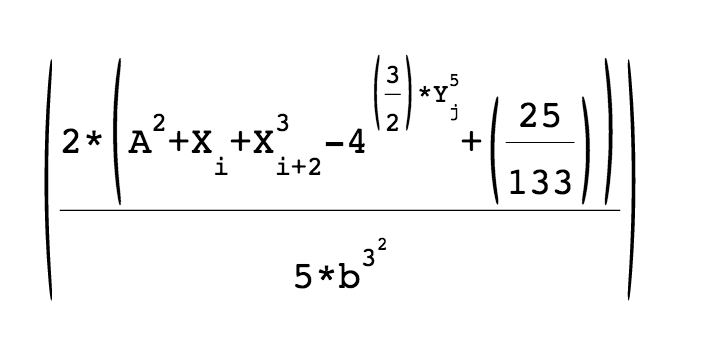
\includegraphics{imgs/i}
        \caption{$(\{2*(A\wedge2+X\_i+X\_\{i+2\}\wedge3-4\wedge\{(3/2)*Y\wedge5\_j\}+(25/133))\}/\{5*b\wedge\{3\wedge2\}\})$}
       \end{centering}
\end{figure}

\indent Este último ejemplo sirve para ver la traducción de una combinación de las distintas operaciones posibles que nos permite la gramática.\\

\newpage
\section{Casos de Prueba}

\indent En el archivo \textbf{tests.py} se encuentran unos pequeños casos de prueba.
\indent Para correrlos, ejecutar en una línea de comandos:
\begin{verbatim}
   python tests.py
\end{verbatim}

\section{Instrucciones de Uso y manual de usuario}

\indent \indent Para correr el programa por línea de comandos ejecutar:\\
\begin{verbatim}
   python traductor.py cadena_a_traducir <archivo_salida>
\end{verbatim}
\indent Algunos símbolos especiales deben escaparse en la cadena de entrada por limitaciones de la línea de comandos. 
\indent Alternativamente se puede utilizar \textbf{traductor2.py}:
\begin{verbatim}
   python traductor2.py <archivo_entrada> <archivo_salida>
\end{verbatim}
\indent Éste último solamente lee la primera línea del archivo de entrada y la traduce.\\

\indent Recomendamos fuertemente utilizar Google Chrome para abrir los archivos .svg.\\
\indent Este trabajo de desarrolló y se probó con las herramientas:
\begin{itemize}
\item \textbf{Python}, versión 2.7
\item \textbf{Ply}, versión 3.8
\item \textbf{Google Chrome}
\end{itemize}

\section{Conclusiones}

\indent Este trabajo práctico nos resultó muy útil para entender un poco más de la aplicación de los conceptos de parsing de la materia en la vida real. Si bien es cierto que las herramientas que usamos nos generaron las tablas de parsing, en lo concerniente a la traducción nos vimos obligados a aplicar lo aprendido de gramáticas de atributos y de traducción dirigida por sintaxis.\\


